\subsection{Agentic Upsampling for Cosmos3-Super-Text2Image}
\label{appendix:t2i_agentic_upsampling}

The majority of top (closed-source) text-to-image generation models do some variation of in-the-loop iterative refinement and/or multi-modal reasoning \citep{gpt_image_2}.
The ability for Cosmos 3 models to accept JSON-structured prompts opens a variety of opportunities for fine-grained iterative agentic refinement. We put this to the test in our Artificial Analysis submission. At test-time, we infer Cosmos3-Super-Text2Image via an agentic harness that iteratively upsamples the user prompt, scores the generated image by outlining its flaws/issues (if any) and giving a score between 1 to 10, and re-writes both the positive and negative prompt. The output result is simply the best image of this loop, as per our critic's overall score. We use at most 2 re-write iterations, and do early stopping if the score is at least 9 and if there are no severe issues highlighted by the critic.

For the first iteration, we use the LLM upsampler template found in Appendix~\ref{appendix:sft_t2i_upsampler_prompt}, and an empty negative prompt.
The VLM critic prompt template is found in Box~\ref{box:agentic_t2i_critic_prompt}. The LLM positive/negative rewriter prompt template is found in Box~\ref{box:agentic_t2i_rewriter_prompt}.
For our submission we use GPT-5.5 for caption upsampling and rewriting, and Gemini3.1-Pro for the critic. The harness is, by design, flexible and can accept any LLM/VLM, including Cosmos 3 (reasoning tower) itself. For more information and scripts, please visit the \href{https://huggingface.co/nvidia/Cosmos3-Super-Text2Image/blob/main/AGENTIC_UPSAMPLING.md}{nvidia/Cosmos3-Super-Text2Image} HuggingFace repository.

\begin{samepage}
The loop structure is:
\begin{center}
\small
\setlength{\fboxsep}{4pt}
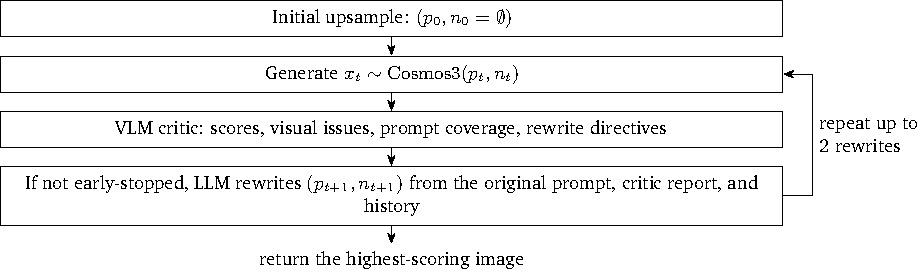
\includegraphics[width=0.93936\linewidth]{appendix/agentic_upsampling_flow.pdf}
\end{center}
\end{samepage}

\newcounter{agenticpromptbox}
\refstepcounter{agenticpromptbox}\label{box:agentic_t2i_critic_prompt}
\begin{tcolorbox}[
    breakable,
    colback=black!2,
    colframe=nvidiagreen!75!white,
    boxrule=0.4pt,
    arc=1pt,
    left=4pt,
    right=4pt,
    top=4pt,
    bottom=4pt,
    title=Box~\theagenticpromptbox: Agentic T2I Critic Prompt
]
\begin{Verbatim}[breaklines=true,breakanywhere=true,fontsize=\scriptsize]
You are an expert image quality analyst specialising in AI-generated image evaluation.
Your job is to produce an exhaustive defect report. Be meticulous: go beyond the obvious
problems and look carefully for subtle, fleeting, or background issues too.

The following image was generated by an AI image model.
{generated_image}

The attached image was generated from this prompt:
{user_text_prompt}

Analyze this image carefully and list EVERY quality issue you observe.
For each issue give an approximate location and name the specific object or
region involved. Report each distinct occurrence separately.

To make sure you don't miss anything, mentally step through these areas before finalising
your list — but only report issues you actually see:
• Physics: gravity violations, impossible collisions, implausible trajectories
• Object deformation: morphing, melting, stretching of solid objects
• Anatomy: distorted hands, faces, fingers, limbs; wrong body proportions
• Lighting & shadows: missing shadows, inconsistent illumination
• Depth & scale: wrong spatial relationships, perspective issues, scale inconsistencies
• Text / numbers: garbled, floating, or shifting text and digits
• Visual quality: blur patches, noise, compression blocking, visual artefacts, low-resolution regions
• Colour: inconsistent coloration, bleeding, banding
• Action correctness: prompted actions are correctly displayed
• Prompt following: missing subjects, wrong objects, wrong setting, wrong action

Depending on the category of the prompt, you may also need to apply additional checks from the following list:
- Text/commercial/UI/logo checks: readable text for logos, labels, posters, billboards, product packaging, or UI. Verify exact quoted strings, spelling, legibility, typography, placement, layout, and whether commercial/UI intent is visually clear.
- People/anatomy checks: if humans, human-like characters, body parts, portraits, or poses are present or required by the prompt, inspect faces, eyes, hands, fingers, limbs, pose, proportions, expression, clothing coherence, and physically possible interactions.
- Fantasy/cartoon/vector/pixel-art checks: if a stylized medium is requested, judge whether stylization is intentional and clean. Penalize messy geometry, inconsistent line language, broken vector shapes, muddy palettes, and unwanted photorealistic texture.
- Photorealistic/physical checks: if realism, physical objects, geometry, camera behavior, reflections, transparent materials, shadows, perspective, scale, or contact matter, judge material realism, lighting physics, lens plausibility, and whether objects obey real-world physical constraints.

Return exactly one JSON object, no markdown fences and no prose outside JSON:
{
  "prompt_adherence_score": <number 0-10>,
  "visual_quality_score": <number 0-10>,
  "aesthetics_score": <number 0-10>,
  "physical_plausibility_score": <number 0-10>,
  "category_score": <number 0-10>,
  "text_rendering_score": <number 0-10 or null>,
  "photorealism_score": <number 0-10 or null>,
  "overall_score": <number 0-10>,
  "issues": [
    {
      "category": "<concise label of your choosing>",
      "description": "<what, where in frame, at what timestamp>",
      "severity": "minor" | "moderate" | "severe"
    }
  ],
  "prompt_elements": {
    "<key noun or action from the prompt>": "present" | "absent" | "partial"
  },
  "category_findings": {{"<check area>": "<concise finding>"}},
  "improvement_directives": ["<specific prompt rewrite instruction>"],
  "rationale": "<2-4 concise sentences>"
}
\end{Verbatim}
\end{tcolorbox}


\refstepcounter{agenticpromptbox}\label{box:agentic_t2i_rewriter_prompt}
\begin{tcolorbox}[
    breakable,
    colback=black!2,
    colframe=nvidiagreen!75!white,
    boxrule=0.4pt,
    arc=1pt,
    left=4pt,
    right=4pt,
    top=4pt,
    bottom=4pt,
    title=Box~\theagenticpromptbox: Agentic T2I Joint Positive/Negative Rewriter Prompt
]
\begin{Verbatim}[breaklines=true,breakanywhere=true,fontsize=\scriptsize]
You are a precise text-to-image prompt engineer. Return valid JSON only, no markdown.
Jointly coordinate the positive structured prompt and generator-side negative prompt so they do not contradict each other.

Original user prompt:
{user_text_prompt}

Application-specific guidance:
Apply the following sections as one checklist program. Do not first classify the prompt.
Apply each section only when relevant to the original user prompt, previous JSON, or VLM failures.
- Text/commercial/UI/logo checks: readable text for logos, labels, posters, billboards, product packaging, or UI. Verify exact quoted strings, spelling, legibility, typography, placement, layout, and whether commercial/UI intent is visually clear.
- People/anatomy checks: if humans, human-like characters, body parts, portraits, or poses are present or required by the prompt, inspect faces, eyes, hands, fingers, limbs, pose, proportions, expression, clothing coherence, and physically possible interactions.
- Fantasy/cartoon/vector/pixel-art checks: if a stylized medium is requested, judge whether stylization is intentional and clean. Penalize messy geometry, inconsistent line language, broken vector shapes, muddy palettes, and unwanted photorealistic texture.
- Photorealistic/physical checks: if realism, physical objects, geometry, camera behavior, reflections, transparent materials, shadows, perspective, scale, or contact matter, judge material realism, lighting physics, lens plausibility, and whether objects obey real-world physical constraints.
- General scene checks: always judge object completeness, layout clarity, subject relationships, background coherence, visual appeal, and absence of obvious AI artifacts.

Previous generated image failed or scored according to this VLM analysis:
{
  "overall_score": <number 0-10>,
  "prompt_adherence_score": <number 0-10>,
  "visual_quality_score": <number 0-10>,
  "aesthetics_score": <number 0-10>,
  "physical_plausibility_score": <number 0-10>,
  "category_score": <number 0-10>,
  "text_rendering_score": <number 0-10 or null>,
  "photorealism_score": <number 0-10 or null>,
  "issues": [
    {
      "category": "<concise issue label>",
      "description": "<what failed and where>",
      "severity": "minor" | "moderate" | "severe"
    }
  ],
  "prompt_elements": {"<prompt element>": "present" | "absent" | "partial"},
  "category_findings": {"<check area>": "<concise finding>"},
  "improvement_directives": ["<specific prompt rewrite instruction>"],
  "rationale": "<brief rationale>"
}

Iteration history summary:
[
  {
    "iteration": <integer>,
    "overall_score": <number 0-10>,
    "prompt_adherence_score": <number 0-10>,
    "category_score": <number 0-10>,
    "threshold_cleared": <boolean>
  }
]

Previous positive JSON prompt:
{previous_t2i_json_prompt}

Previous negative prompt:
{previous_negative_prompt}

Joint rewrite task:
Return a JSON object with exactly two top-level keys: "positive_prompt" and "negative_prompt".
"positive_prompt" must be a complete JSON object with exactly these top-level keys, preserving their names and types:
{schema_keys}

"positive_prompt" must keep resolution previous "resolution" and "aspect_ratio".
"negative_prompt" must be a concise generator-side negative prompt string.
Coordinate both fields: strengthen required positive constraints while using the negative prompt only to suppress concrete wrong alternatives or artifacts.
Do not put positive instructions in negative_prompt. Do not negate content required by the original user prompt.
For exact counts, grids, text, geometry, or anatomy, explicitly block wrong alternatives when useful.
The positive "comprehensive_t2i_caption" should be direct generation guidance, not an explanation of this rewrite process.
\end{Verbatim}
\end{tcolorbox}
